\section{Experiment}
    \subsection{Data Preprocessing}
        \begin{figure}[tbh]
            \centering
            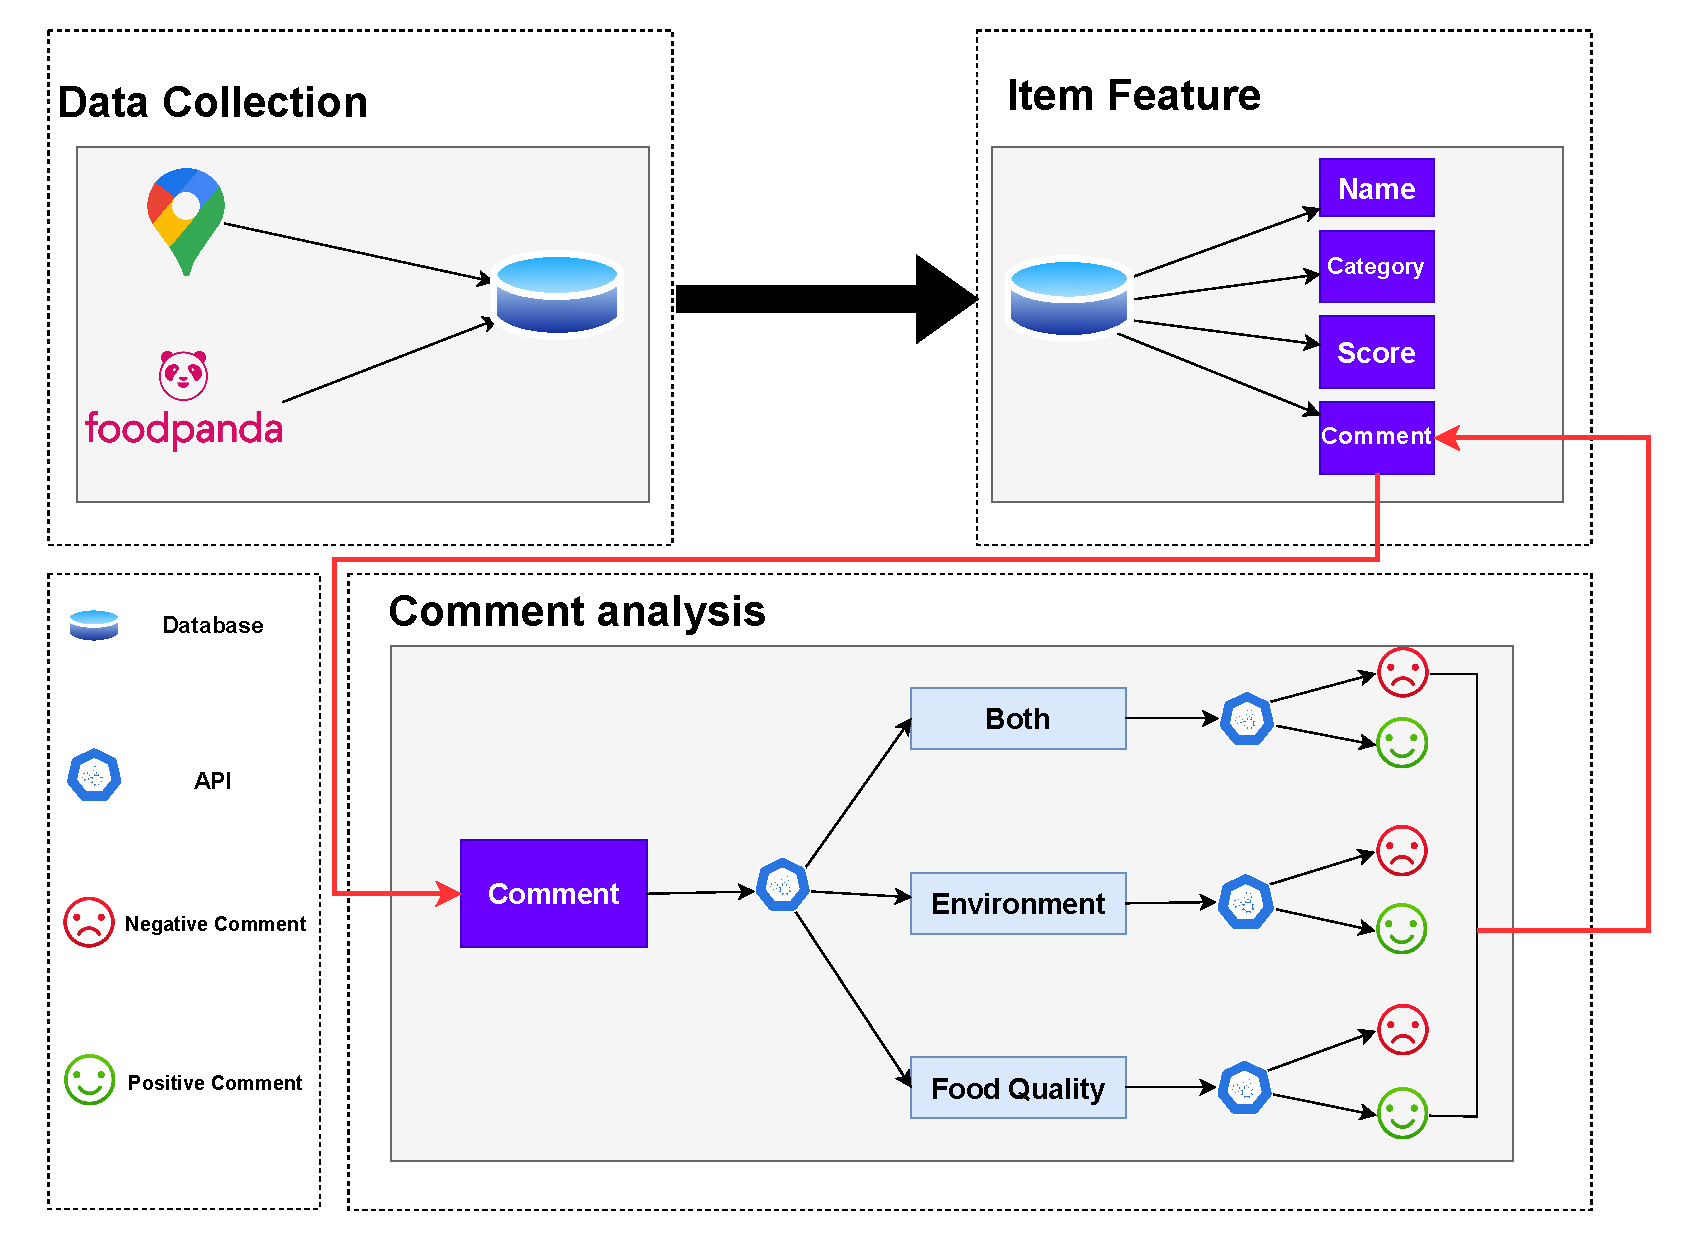
\includegraphics[width=0.5\textwidth]{img/preprocess.pdf}
            \caption{資料前處理架構圖}
            \label{fig-preprocess}
        \end{figure}
        本研究的資料前處理架構如 \xfig{fig-preprocess} 所示,利用爬蟲技術從 Foodpanda 和 Google Maps 獲取餐廳資料。每間餐廳的資料涵蓋了餐廳名稱、餐廳類型、評分以及顧客的評論。由於每家店通常會累積大量的評論,這些評論內容對於描述店家的品質、服務及顧客的體驗具有高度相關性。若將所有評論合併後再丟入大規模語言模型(LLM)進行分析,可能會因評論主題多樣性導致訊息混雜,進而影響模型的微調(Fine Tuning)效果。當不同主題的評論一起進行訓練時,模型可能難以識別每個特徵的意圖,進而影響結果的精準度。

        為提升模型的針對性,本研究首先將評論依主題分為三類:餐點品質、店內環境氣氛,以及兩者皆有的綜合評價。針對這三類評論,我們分別對每一類進行獨立的 LLM 微調。這種獨立的微調方法有助於每個模型專注於該主題的特徵,避免不同主題之間的訊息干擾。對於餐點品質類評論,模型學習專注於食物的口感、質量及呈現;對於店內環境氣氛的評論,模型則聚焦在用餐氛圍、環境設計及舒適度等描述上;而綜合評價類別則幫助模型掌握顧客的整體體驗。通過分開微調,每個模型能精確捕捉該主題的特徵表現,使得每一類評論的處理結果更具針對性。

        完成初步主題分類與獨立微調後,針對每一類主題中的評論再進行情感分析,以判斷其情感取向為正面或負面。這一分層且分主題的處理架構,能夠生成更為精確的特徵向量,使得每條評論的語意信息充分表達,進一步提升了推薦系統的精準度和可靠性。
\color{black}